\vspace{-5pt}
\section{Introduction}
\label{sec:intro}
\vspace{-2pt}
During the last few years, self-supervised learning (SSL) has become the most popular paradigm for unsupervised visual representation learning \cite{caron2020unsupervised, caron2021emerging, chen2020simple, he2020momentum, grill2020bootstrap, zbontar2021barlow, bardes2021vicreg, chen2020improved}. Indeed, under certain assumptions (\textit{e.g.}, offline training with large amounts of data and resources), SSL methods are able to extract representations that match the quality of representations obtained with supervised learning, without requiring annotations. However, these assumptions do not always hold in real-world scenarios, \textit{e.g.}, when new unlabeled data are made available progressively over time.
In fact, in order to integrate new knowledge into the model, training needs to be repeated on the whole dataset, which is impractical, expensive, and sometimes even impossible when old data is not available. This issue is exacerbated by the fact that SSL models are notoriously computationally expensive to train.

\begin{figure}[t]
\centering
\vspace{-5pt}
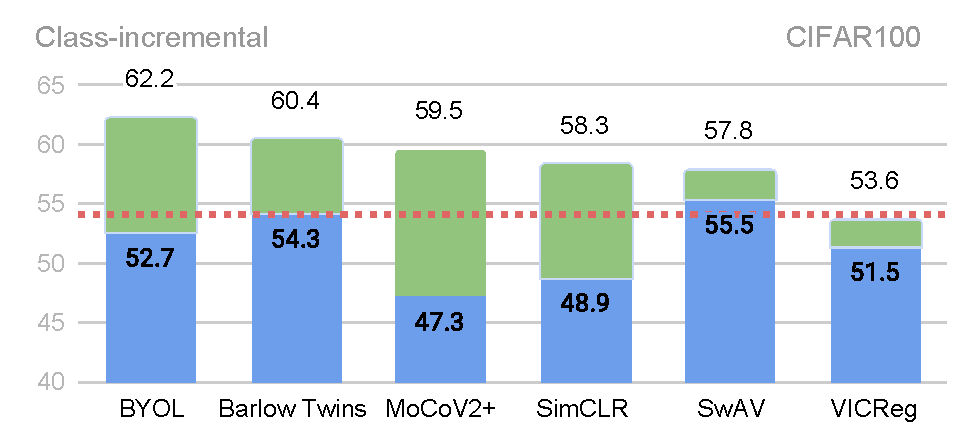
\includegraphics[width=0.99\columnwidth]{figures/cifar100.pdf}
\vspace{-12pt}
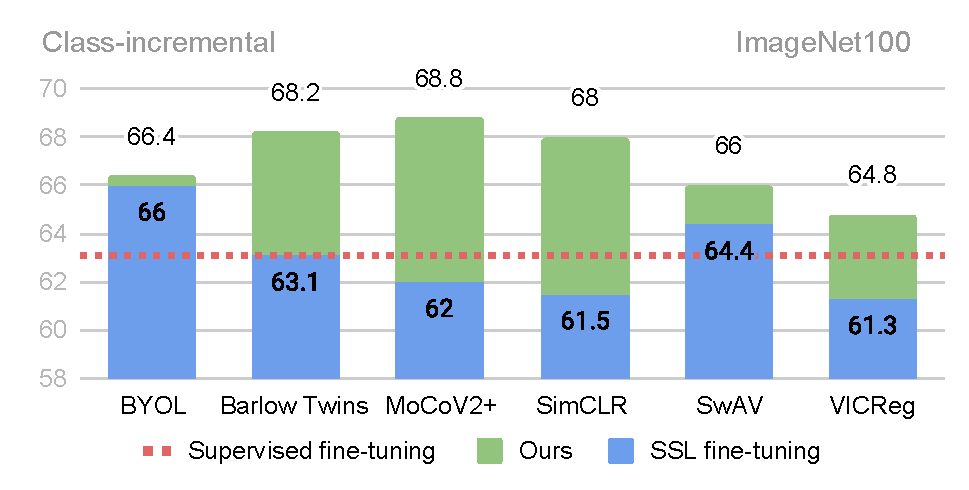
\includegraphics[width=0.99\columnwidth]{figures/im100.pdf}
\caption{Linear evaluation accuracy of representations learned with different self-supervised methods on class-incremental CIFAR100 and ImageNet100. In blue the accuracy of SSL fine-tuning, in green the improvement brought by \name{}. The red  dashed line is the accuracy attained by supervised fine-tuning.}
\vspace{-15pt}
\label{fig:teaser}
\end{figure}


Continual learning (CL) studies the ability of neural networks to learn tasks sequentially. Prior art in the field focuses on mitigating {catastrophic forgetting}~\cite{Mccloskey89,French99, Goodfellow13,de2019continual}. Common benchmarks in the CL literature evaluate the discriminative performance of classifiers learned \emph{with supervision} from non-stationary distributions. 
In this paper, we tackle the same forgetting phenomenon in the context of SSL. 
Unsupervised representation learning is indeed appealing for sequential learning since it does not require human annotations, which are particularly hard to obtain when new data is generated on-the-fly. This setup, called Continual Self-Supervised Learning (CSSL), is surprisingly under-investigated in the literature.

In this work, we propose \name{}, a simple and effective framework for CSSL of visual representations based on the intuition that SSL models are intrinsically capable of learning continually, and that SSL losses can be seamlessly converted into distillation losses. Our key idea is to train the current model to predict past representations with
a prediction head, thus encouraging it to remember past knowledge. \name{} has several favourable features: (i) it is compatible with popular state-of-the-art SSL loss functions and architectures, (ii) it is simple to implement, and (iii) it does not require any additional hyperparameter tuning with respect to the original SSL method. Our experiments demonstrate that SSL methods trained continually with \name{} significantly outperform all the related methods (CSSL baselines and several methods adapted from supervised CL).

We also perform a comprehensive analysis of the behavior of six popular SSL methods in diverse CL settings (\ie, class, data, and domain incremental). We provide empirical results on small (CIFAR100), medium (ImageNet100), and large (DomainNet) scale datasets. 
Our study sheds new light on interesting properties of SSL methods that emerge when learning continually.
Among other findings, we discover that, in the class-incremental setting, SSL methods typically approach or outperform supervised learning (see Fig.\ref{fig:teaser}), while this is not generally true for other settings (data-incremental and domain-incremental) where supervised learning still shows a sizeable advantage.
